% =============================================================================
% Semana 12 — Apresentação em Grupo: Dashboard Storytelling no Tableau
% Aula de 3 horas (19h–22h) | 18/05/2026 — última aula antes das provas
% =============================================================================

\chapter{Semana 12 (18/05/2026) — Apresentação em Grupo: Dashboard Storytelling}

% ---------------------------------------------------------------------------
\section{Objetivo e Contexto}
% ---------------------------------------------------------------------------

\begin{NoteBox}
\textbf{Esta é a última aula antes da semana de provas (25/05).}

Cada grupo receberá um dataset real do Kaggle, uma dor de negócio, uma pergunta
norteadora e um protótipo de dashboard. A missão: construir um dashboard no Tableau
que \textbf{force uma decisão} — não apenas exiba dados — e apresentar em
\textbf{3 minutos} no formato pitch (Situação → Complicação → Resolução → Próximo passo).

\textbf{Requisito obrigatório:} incluir ao menos um \textbf{Insight gerado por IA}
(ChatGPT / Gemini) posicionado ao lado do Big Number no dashboard.
\end{NoteBox}

\begin{BoardBox}
\textbf{Roteiro da aula (19h–22h)}
\begin{enumerate}
  \item 19h–19h20 — \textbf{Briefing:} divisão de grupos + entrega de datasets + instruções
  \item 19h20–19h40 — \textbf{Teoria rápida:} boas práticas de storytelling + estrutura do dashboard
  \item 19h40–21h20 — \textbf{Construção guiada:} cada grupo monta seu dashboard no Tableau
  \item 21h20–21h50 — \textbf{Apresentações:} pitch de 3 min por grupo (5 grupos × 6 min)
  \item 21h50–22h — \textbf{Feedback coletivo + orientações finais para as provas}
\end{enumerate}
\end{BoardBox}

% =============================================================================
\section{Teoria Rápida — Boas Práticas de Storytelling (19h20–19h40)}
% =============================================================================

\begin{BoardBox}
\textbf{Estrutura obrigatória do dashboard (para o quadro)}

Todo dashboard desta aula deve seguir a estrutura abaixo, repetindo o bloco
``Pergunta → Big Number + Insight IA → Gráficos'' para cada pergunta de negócio:

\medskip
\begin{tabular}{|p{13cm}|}
\hline
\textbf{[PERGUNTA DE NEGÓCIO]} \\
\hline
\textbf{Big Number} (coluna esquerda) \quad|\quad \textbf{Insight IA} (coluna direita) \\
\hline
\textbf{Gráfico 1} \quad|\quad \textbf{Gráfico 2} \\
(respondem à pergunta acima) \\
\hline
\textbf{[PRÓXIMA PERGUNTA DE NEGÓCIO]} \\
\hline
\textbf{Gráfico 3} \quad|\quad \textbf{Gráfico 4} \\
\hline
\textbf{TABELA ANALÍTICA FINAL} (largura total) \\
\hline
\end{tabular}

\medskip
O Call to Action deve aparecer como título do dashboard ou como painel de texto
no rodapé — nunca oculto em alguma aba.
\end{BoardBox}

\begin{SolvedBox}
\textbf{Checklist de boas práticas que DEVEM aparecer no dashboard:}

\begin{enumerate}
  \item \textbf{Cor com propósito:} 1 cor de destaque (ex.: laranja) para o dado que carrega
  a mensagem; tudo mais em cinza ou azul neutro. Sem arco-íris.
  \item \textbf{Título-mensagem em cada gráfico:} não ``Gráfico de Barras'' — sim
  ``Eletrônicos têm 2,4$\times$ mais atrasos que a média''.
  \item \textbf{Big Number prominente:} número grande, fonte $\geq$ 24pt, com rótulo descritivo
  abaixo e indicador de gap em relação à meta (seta ▲▼ + delta pp ou \%).
  \item \textbf{Insight IA ao lado do Big Number:} painel de texto com o insight gerado
  pela IA em itálico, delimitado por aspas e com rótulo ``[Insight IA]''.
  \item \textbf{Hierarquia Z:} elemento mais importante no canto superior esquerdo;
  Call to Action no rodapé ou no topo como subtítulo da pergunta.
  \item \textbf{Data-ink ratio:} sem grades pesadas, sem 3D, sem sombras, sem gradientes
  decorativos. Cada pixel deve carregar dado.
  \item \textbf{Tabela analítica no final:} mostra os dados brutos consolidados para
  quem quiser detalhe — não substitui os gráficos.
  \item \textbf{Interatividade mínima:} ao menos 1 filtro ou parâmetro funcionando no
  dashboard (ex.: filtro por período ou parâmetro de Top N).
\end{enumerate}
\end{SolvedBox}

% ---------------------------------------------------------------------------
\subsection{Pré-atenção e Cognição — Decisões de Design em 30 Segundos}
% ---------------------------------------------------------------------------

\begin{SolvedBox}
\textbf{Como o cérebro processa o dashboard — guia de decisões de design:}

\begin{tabular}{|p{3cm}|p{5cm}|p{5.5cm}|}
\hline
\textbf{Princípio} & \textbf{O que fazer} & \textbf{Erro comum} \\
\hline
Cor semântica & Vermelho = alerta; Verde = ok; Laranja = atenção & Usar vermelho para a cor-tema do dashboard \\
\hline
Contraste & Fundo claro + texto escuro; 1 cor viva & Texto cinza-claro em fundo branco \\
\hline
Proximidade & Título do gráfico imediatamente acima do visual & Título distante do gráfico que descreve \\
\hline
Alinhamento & Grade consistente; colunas alinhadas & Visuais em tamanhos diferentes sem razão \\
\hline
Consistência & Região Sul sempre azul em todas as telas & Azul na tela 1, verde na tela 2 para o mesmo item \\
\hline
Limite atencional & Máx. 5 elementos focais por tela & 12 KPIs sem prioridade = 0 KPIs \\
\hline
\end{tabular}
\end{SolvedBox}

\begin{BoardBox}
\textbf{Como criar o Insight IA — passo a passo (para o quadro)}

\begin{enumerate}
  \item No Tableau, exporte ou copie os dados principais (ex.: top 10 linhas + métricas).
  \item Abra o ChatGPT ou o Gemini e use o prompt abaixo:
\end{enumerate}

\medskip
\begin{quote}
\textit{``Você é um analista de dados sênior. Com base nos dados abaixo, gere UM insight
acionável em 2-3 linhas. O insight deve: (1) identificar um padrão não óbvio, (2)
quantificar o impacto e (3) sugerir uma ação concreta com estimativa de resultado.
Dados: [cole aqui os dados do seu grupo]. Contexto do negócio: [descreva a dor do
seu grupo em 1 frase].''}
\end{quote}

\medskip
\begin{enumerate}
  \setcounter{enumi}{2}
  \item Copie a resposta da IA para um painel de texto no Tableau.
  \item Formate em itálico, delimite com aspas e adicione o rótulo \textbf{[Insight IA]}.
  \item Posicione ao lado direito do Big Number.
\end{enumerate}
\end{BoardBox}

% =============================================================================
\section{Divisão de Grupos}
% =============================================================================

\begin{BoardBox}
\textbf{Grupos da turma — sorteio ou designação pelo professor}

\begin{tabular}{|l|p{3.5cm}|p{3cm}|p{3cm}|}
\hline
\textbf{Grupo} & \textbf{Dataset} & \textbf{Integrantes} & \textbf{Link Kaggle} \\
\hline
Grupo 1 & E-commerce (Olist) & & kaggle.com/olistbr/... \\
Grupo 2 & People Analytics (IBM HR) & & kaggle.com/pavansubhasht/... \\
Grupo 3 & Varejo (Superstore) & & kaggle.com/vivek468/... \\
Grupo 4 & Saúde (Heart Disease) & & kaggle.com/johnsmith88/... \\
Grupo 5 & Fintech (Credit Card) & & kaggle.com/sakshigoyal7/... \\
\hline
\end{tabular}
\end{BoardBox}

% =============================================================================
\section{Grupo 1 — E-commerce: Olist Brazilian E-Commerce}
% =============================================================================

\begin{BoardBox}
\textbf{Briefing do Grupo 1}

\textbf{Dataset:} Brazilian E-Commerce Public Dataset (Olist)\\
\textbf{Link:} \url{https://www.kaggle.com/datasets/olistbr/brazilian-ecommerce}

\textbf{Dor de Negócio:} atrasos na entrega derrubam as avaliações dos clientes
e aumentam o churn de vendedores parceiros da plataforma.

\textbf{Pergunta 1:} ``Em quais estados e categorias de produto os atrasos são mais
críticos e qual o impacto nas avaliações (review\_score)?''

\textbf{Pergunta 2:} ``Como o tempo de entrega (dias) se correlaciona com o
review\_score do cliente?''

\textbf{Big Idea sugerida:} ``Eletrônicos em SP concentram 34\% dos atrasos e puxam
o review médio para 3,2 estrelas — priorizar logística nessa categoria pode aumentar
o review para 4,1 e reduzir o churn de vendedores em 15\%.''

\textbf{Call to Action:} redesenhar a rota logística de Eletrônicos em SP até o Q3 2026.
\end{BoardBox}

\begin{SolvedBox}
\textbf{Transformações necessárias no dataset (Tableau Prep ou Python):}

O dataset Olist é composto por múltiplos arquivos CSV que precisam ser unidos:
\begin{enumerate}
  \item \textbf{Join principal:} \texttt{orders} $\bowtie$ \texttt{order\_items}
  $\bowtie$ \texttt{products} $\bowtie$ \texttt{customers}
  (chave: \texttt{order\_id} e \texttt{product\_id}).
  \item \textbf{Campo calculado — atraso:}\\
  \texttt{delivery\_delay = order\_delivered\_customer\_date − order\_estimated\_delivery\_date}\\
  Se $> 0$: atraso; se $\leq 0$: entrega no prazo.
  \item \textbf{Campo calculado — status:}\\
  \texttt{is\_late = IF delivery\_delay > 0 THEN "Atrasado" ELSE "No Prazo" END}
  \item \textbf{Tradução de categoria:} usar o arquivo \texttt{product\_category\_name\_translation.csv}
  para mapear nomes em português → inglês (ou manter em PT).
  \item \textbf{Estado do cliente:} extrair \texttt{customer\_state} da tabela \texttt{customers}
  (já disponível como sigla UF — pronto para Geographic Role no Tableau).
  \item \textbf{Filtrar:} remover pedidos com status \texttt{canceled} ou \texttt{unavailable}.
\end{enumerate}

\textbf{Campos para o dashboard:}
\texttt{customer\_state}, \texttt{product\_category\_name}, \texttt{delivery\_delay},
\texttt{is\_late}, \texttt{review\_score}, \texttt{price}, \texttt{order\_purchase\_timestamp}.
\end{SolvedBox}

\begin{SolvedBox}
\textbf{Construção do dashboard no Tableau — passo a passo:}

\textbf{Sheet 1 — Big Number:}
\begin{itemize}
  \item Arrastar \texttt{is\_late} para Filters → selecionar ``Atrasado''
  \item Arrastar \texttt{order\_id} para Texto → mudar para COUNTD
  \item Criar campo calculado: \texttt{\% Atrasados = COUNTD([order\_id onde is\_late=Atrasado]) / COUNTD([order\_id])}
  \item Fonte 28pt, cor laranja — este é o Big Number
\end{itemize}

\textbf{Sheet 2 — Mapa Coroplético (Pergunta 1):}
\begin{itemize}
  \item Arrastar \texttt{customer\_state} para Detail → Geographic Role → State/Province
  \item Arrastar \texttt{is\_late} para Color (filtrar ``Atrasado'') e \texttt{order\_id} para Size
  \item Show Me → Filled Map
  \item Título: ``SP concentra X\% dos atrasos — maior impacto na plataforma''
\end{itemize}

\textbf{Sheet 3 — Barras Horizontais por Categoria:}
\begin{itemize}
  \item Arrastar \texttt{product\_category\_name} para Rows, \texttt{\% Atrasados} para Columns
  \item Ordenar decrescente; destacar a barra da categoria líder em laranja
  \item Título: ``[Categoria X] tem 2,4$\times$ mais atrasos que a média''
\end{itemize}

\textbf{Sheet 4 — Scatter (Pergunta 2):}
\begin{itemize}
  \item Arrastar \texttt{delivery\_delay} para Columns, \texttt{review\_score} (AVG) para Rows
  \item Adicionar linha de tendência: Analytics → Trend Line → Linear
  \item Título: ``Cada dia de atraso reduz o review médio em X pontos''
\end{itemize}

\textbf{Sheet 5 — Linha Temporal:}
\begin{itemize}
  \item Arrastar \texttt{order\_purchase\_timestamp} (Month) para Columns,
  \texttt{is\_late} (COUNT) para Rows, filtrar ``Atrasado''
  \item Adicionar linha de referência com a média
  \item Título: ``Atrasos crescem X\% nos últimos 3 meses''
\end{itemize}

\textbf{Dashboard final:} Q1 header → [Big Number | Insight IA] → [Sheet 2 | Sheet 3]
→ Q2 header → [Sheet 4 | Sheet 5] → Tabela analítica final (Sheet com \texttt{customer\_state},
\texttt{product\_category\_name}, \texttt{\% Atrasados}, \texttt{review\_score} médio).
\end{SolvedBox}

\begin{figure}[H]
\centering
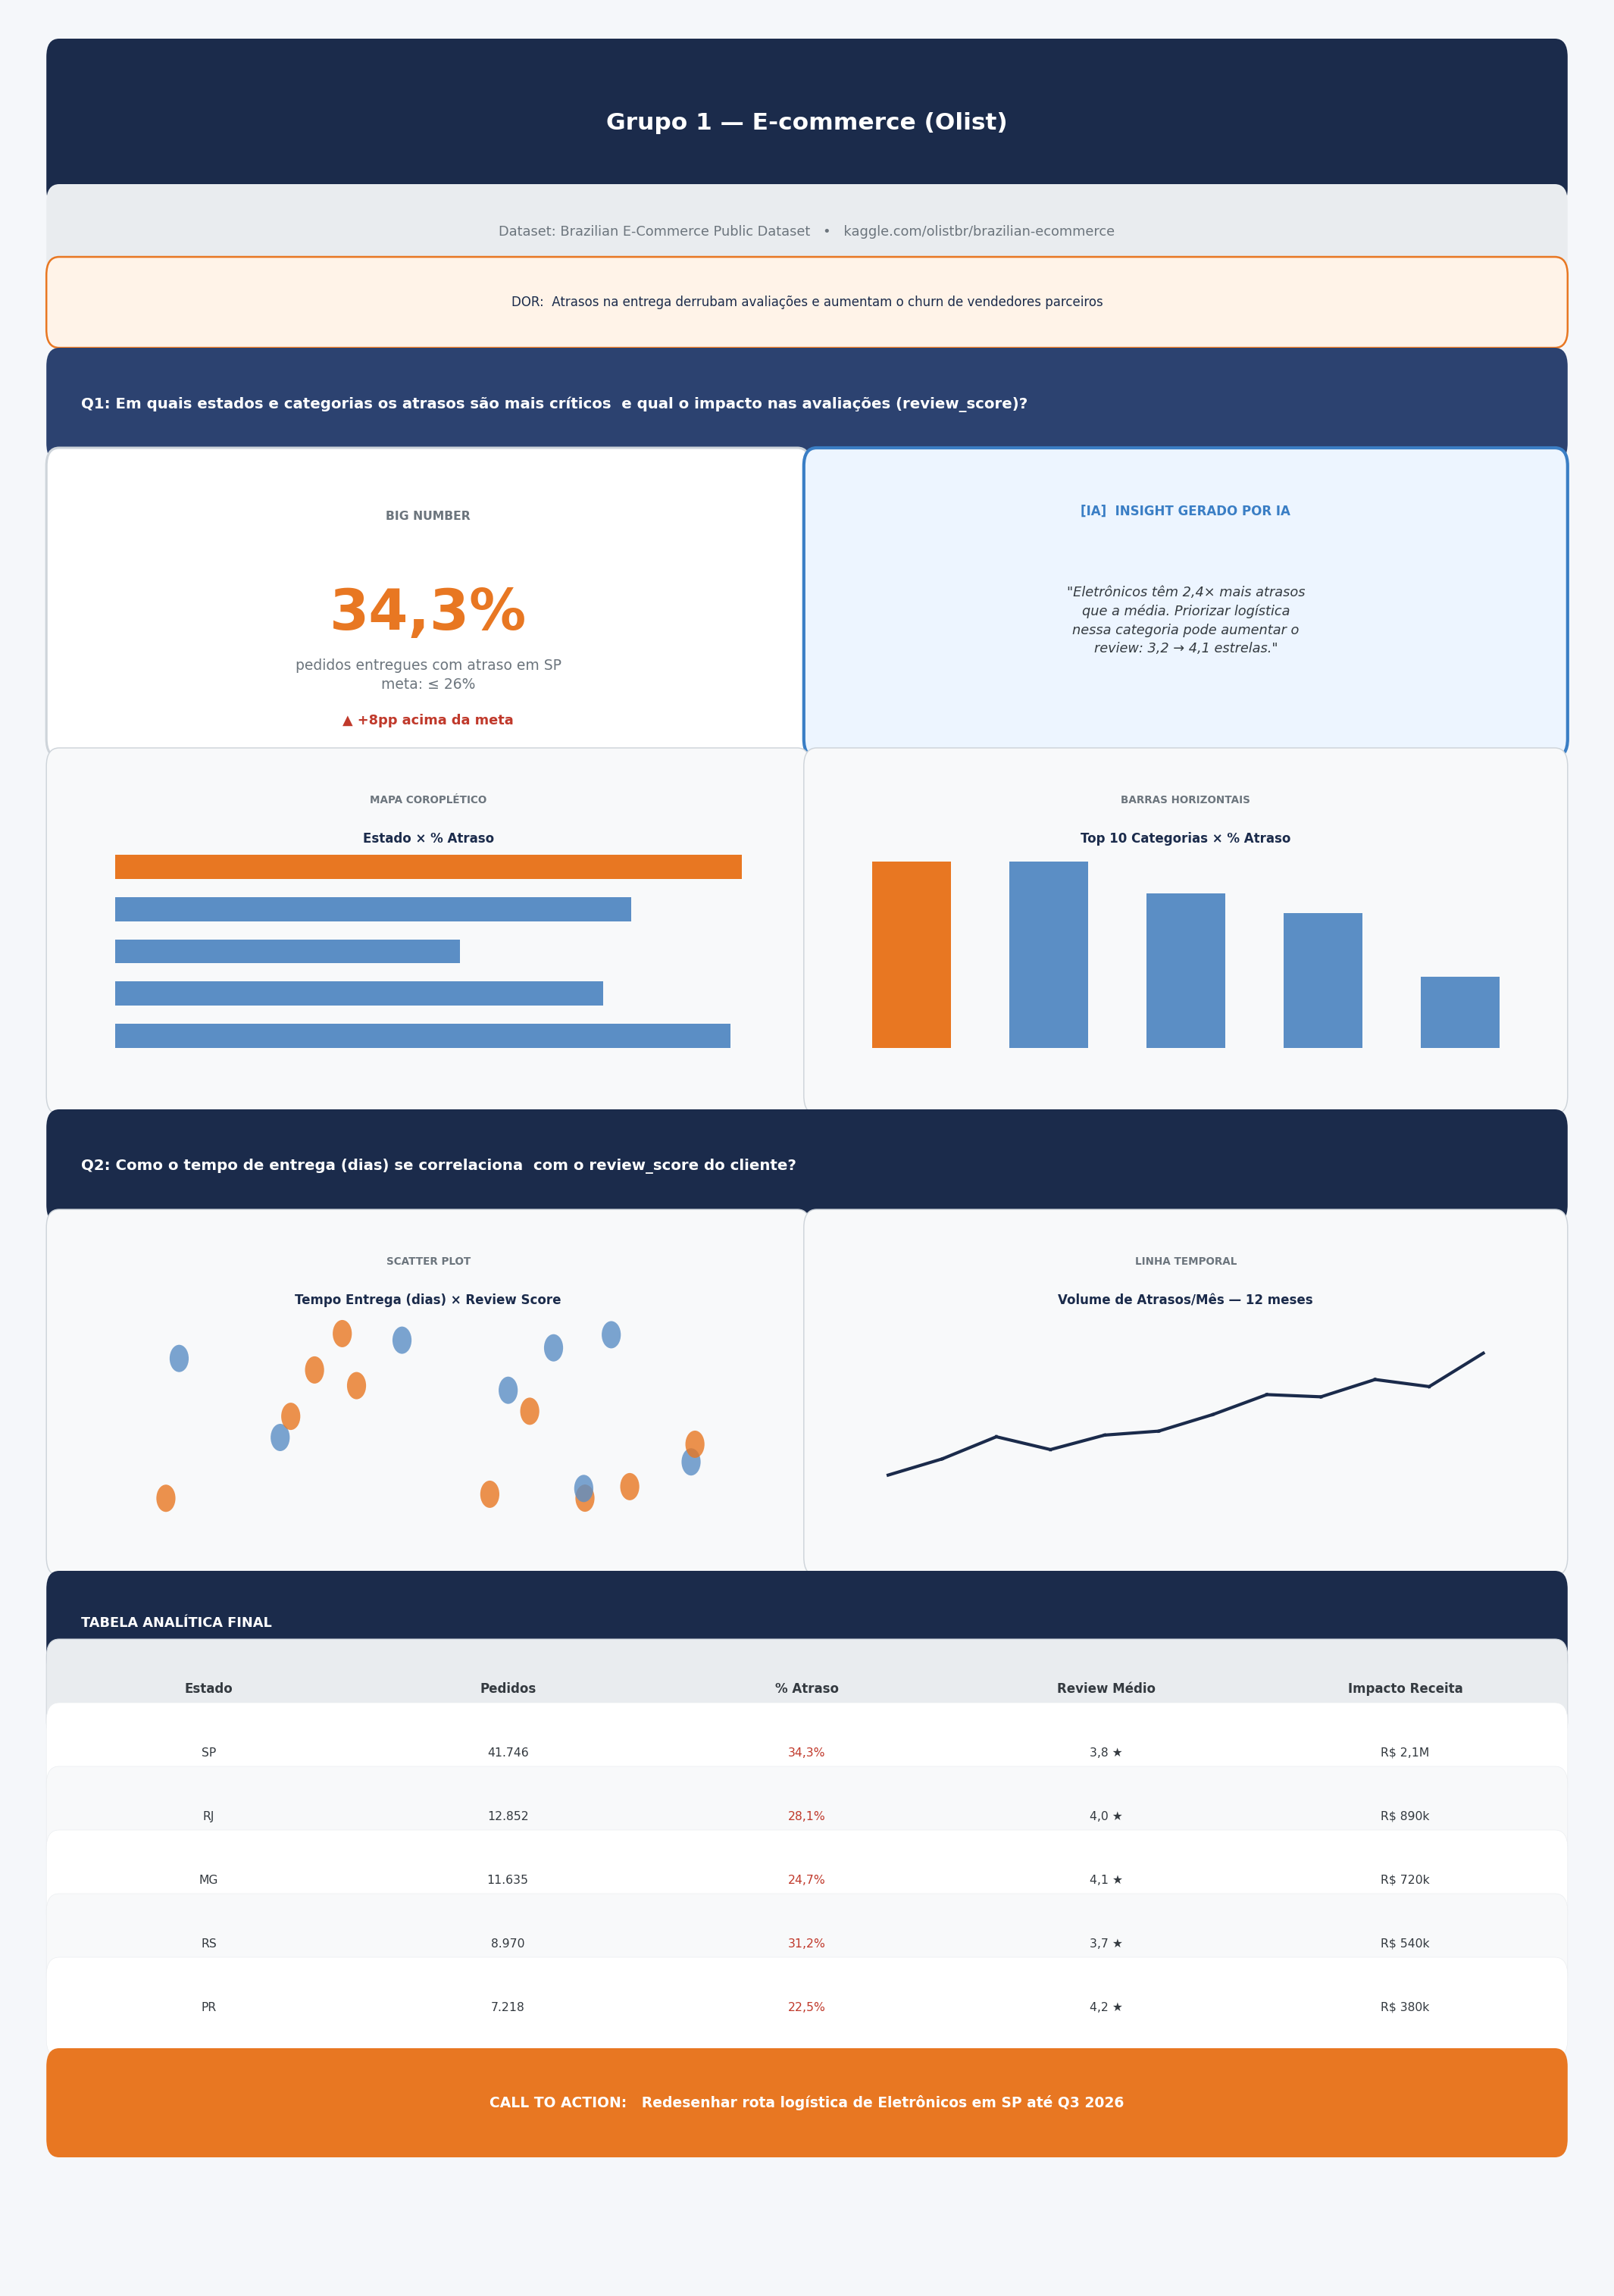
\includegraphics[width=\textwidth]{wireframes/wireframe_grupo1_olist.png}
\caption{Protótipo do dashboard — Grupo 1 (E-commerce Olist). Big Number à esquerda,
Insight IA à direita, gráficos por pergunta, tabela analítica ao final.}
\end{figure}

% =============================================================================
\section{Grupo 2 — People Analytics: IBM HR Employee Attrition}
% =============================================================================

\begin{BoardBox}
\textbf{Briefing do Grupo 2}

\textbf{Dataset:} IBM HR Analytics Employee Attrition \& Performance\\
\textbf{Link:} \url{https://www.kaggle.com/datasets/pavansubhasht/ibm-hr-analytics-attrition-dataset}

\textbf{Dor de Negócio:} turnover de 28\% em TI custa R\$450k/ano em recrutamento e
perda de conhecimento institucional.

\textbf{Pergunta 1:} ``Qual perfil de funcionário tem maior risco de saída e em
qual departamento o problema é mais crítico?''

\textbf{Pergunta 2:} ``Satisfação no trabalho e faixa salarial influenciam
significativamente o turnover?''

\textbf{Big Idea sugerida:} ``Funcionários de TI com menos de 2 anos de empresa e sem
promoção nos últimos 3 anos têm 3$\times$ mais chance de sair — um programa de mentoria
focado nesse perfil pode reduzir o turnover de 28\% para 15\% e economizar R\$270k/ano.''

\textbf{Call to Action:} implantar programa de mentoria para funcionários $<$ 2 anos
em TI e Vendas até junho/2026.
\end{BoardBox}

\begin{SolvedBox}
\textbf{Transformações necessárias (dataset já limpo — arquivo único):}

\begin{enumerate}
  \item \textbf{Variável alvo:} \texttt{Attrition} (Yes/No) → campo calculado binário:
  \texttt{Attrition\_Num = IF [Attrition]="Yes" THEN 1 ELSE 0 END}
  \item \textbf{Taxa de turnover:} \texttt{Turnover\_Rate = AVG(Attrition\_Num) * 100}
  \item \textbf{Faixa salarial:} campo calculado com bins de \texttt{MonthlyIncome}:
  \texttt{IF [MonthlyIncome] < 3000 THEN "Baixo"}
  \texttt{ELSEIF [MonthlyIncome] < 7000 THEN "Médio"}
  \texttt{ELSE "Alto" END}
  \item \textbf{Perfil de risco:} campo calculado:
  \texttt{IF [YearsAtCompany] < 2 AND [YearsSinceLastPromotion] > 2}
  \texttt{THEN "Alto Risco" ELSE "Normal" END}
  \item \textbf{Satisfação combinada:} média de \texttt{JobSatisfaction},
  \texttt{EnvironmentSatisfaction} e \texttt{RelationshipSatisfaction}.
\end{enumerate}

\textbf{Campos para o dashboard:}
\texttt{Department}, \texttt{Attrition}, \texttt{Turnover\_Rate}, \texttt{Faixa\_Salarial},
\texttt{YearsAtCompany}, \texttt{Perfil\_Risco}, \texttt{JobSatisfaction}, \texttt{MonthlyIncome}.
\end{SolvedBox}

\begin{SolvedBox}
\textbf{Construção do dashboard no Tableau:}

\textbf{Sheet 1 — Big Number:} \texttt{AVG(Attrition\_Num)} filtrado por
\texttt{Department = "Research \& Development"} ou TI. Fonte 28pt, laranja.

\textbf{Sheet 2 — Barras por Departamento (Pergunta 1):}
\texttt{Department} nas Rows, \texttt{Turnover\_Rate} nas Columns; ordenar decrescente;
linha de referência com a média geral; destacar o departamento crítico em laranja.
Título: ``[Dept. X]: turnover de Y\% — 2,5$\times$ acima da média''.

\textbf{Sheet 3 — Heatmap Satisfação × Salário × Turnover (Pergunta 1):}
\texttt{Faixa\_Salarial} nas Columns, \texttt{JobSatisfaction} (como dimensão 1–4) nas Rows;
cor por \texttt{AVG(Attrition\_Num)}; escala divergente vermelho-verde.

\textbf{Sheet 4 — Scatter Anos × P(Saída) (Pergunta 2):}
\texttt{YearsAtCompany} nas Columns, \texttt{Turnover\_Rate} nas Rows; cor por
\texttt{Perfil\_Risco}; linha de tendência; título: ``Primeiros 2 anos = zona crítica''.

\textbf{Sheet 5 — Bullet Chart por Departamento:}
\texttt{Turnover\_Rate} atual vs meta de 15\% (parâmetro); mostrar gap por
departamento. Título: ``3 departamentos acima da meta de turnover''.
\end{SolvedBox}

\begin{figure}[H]
\centering
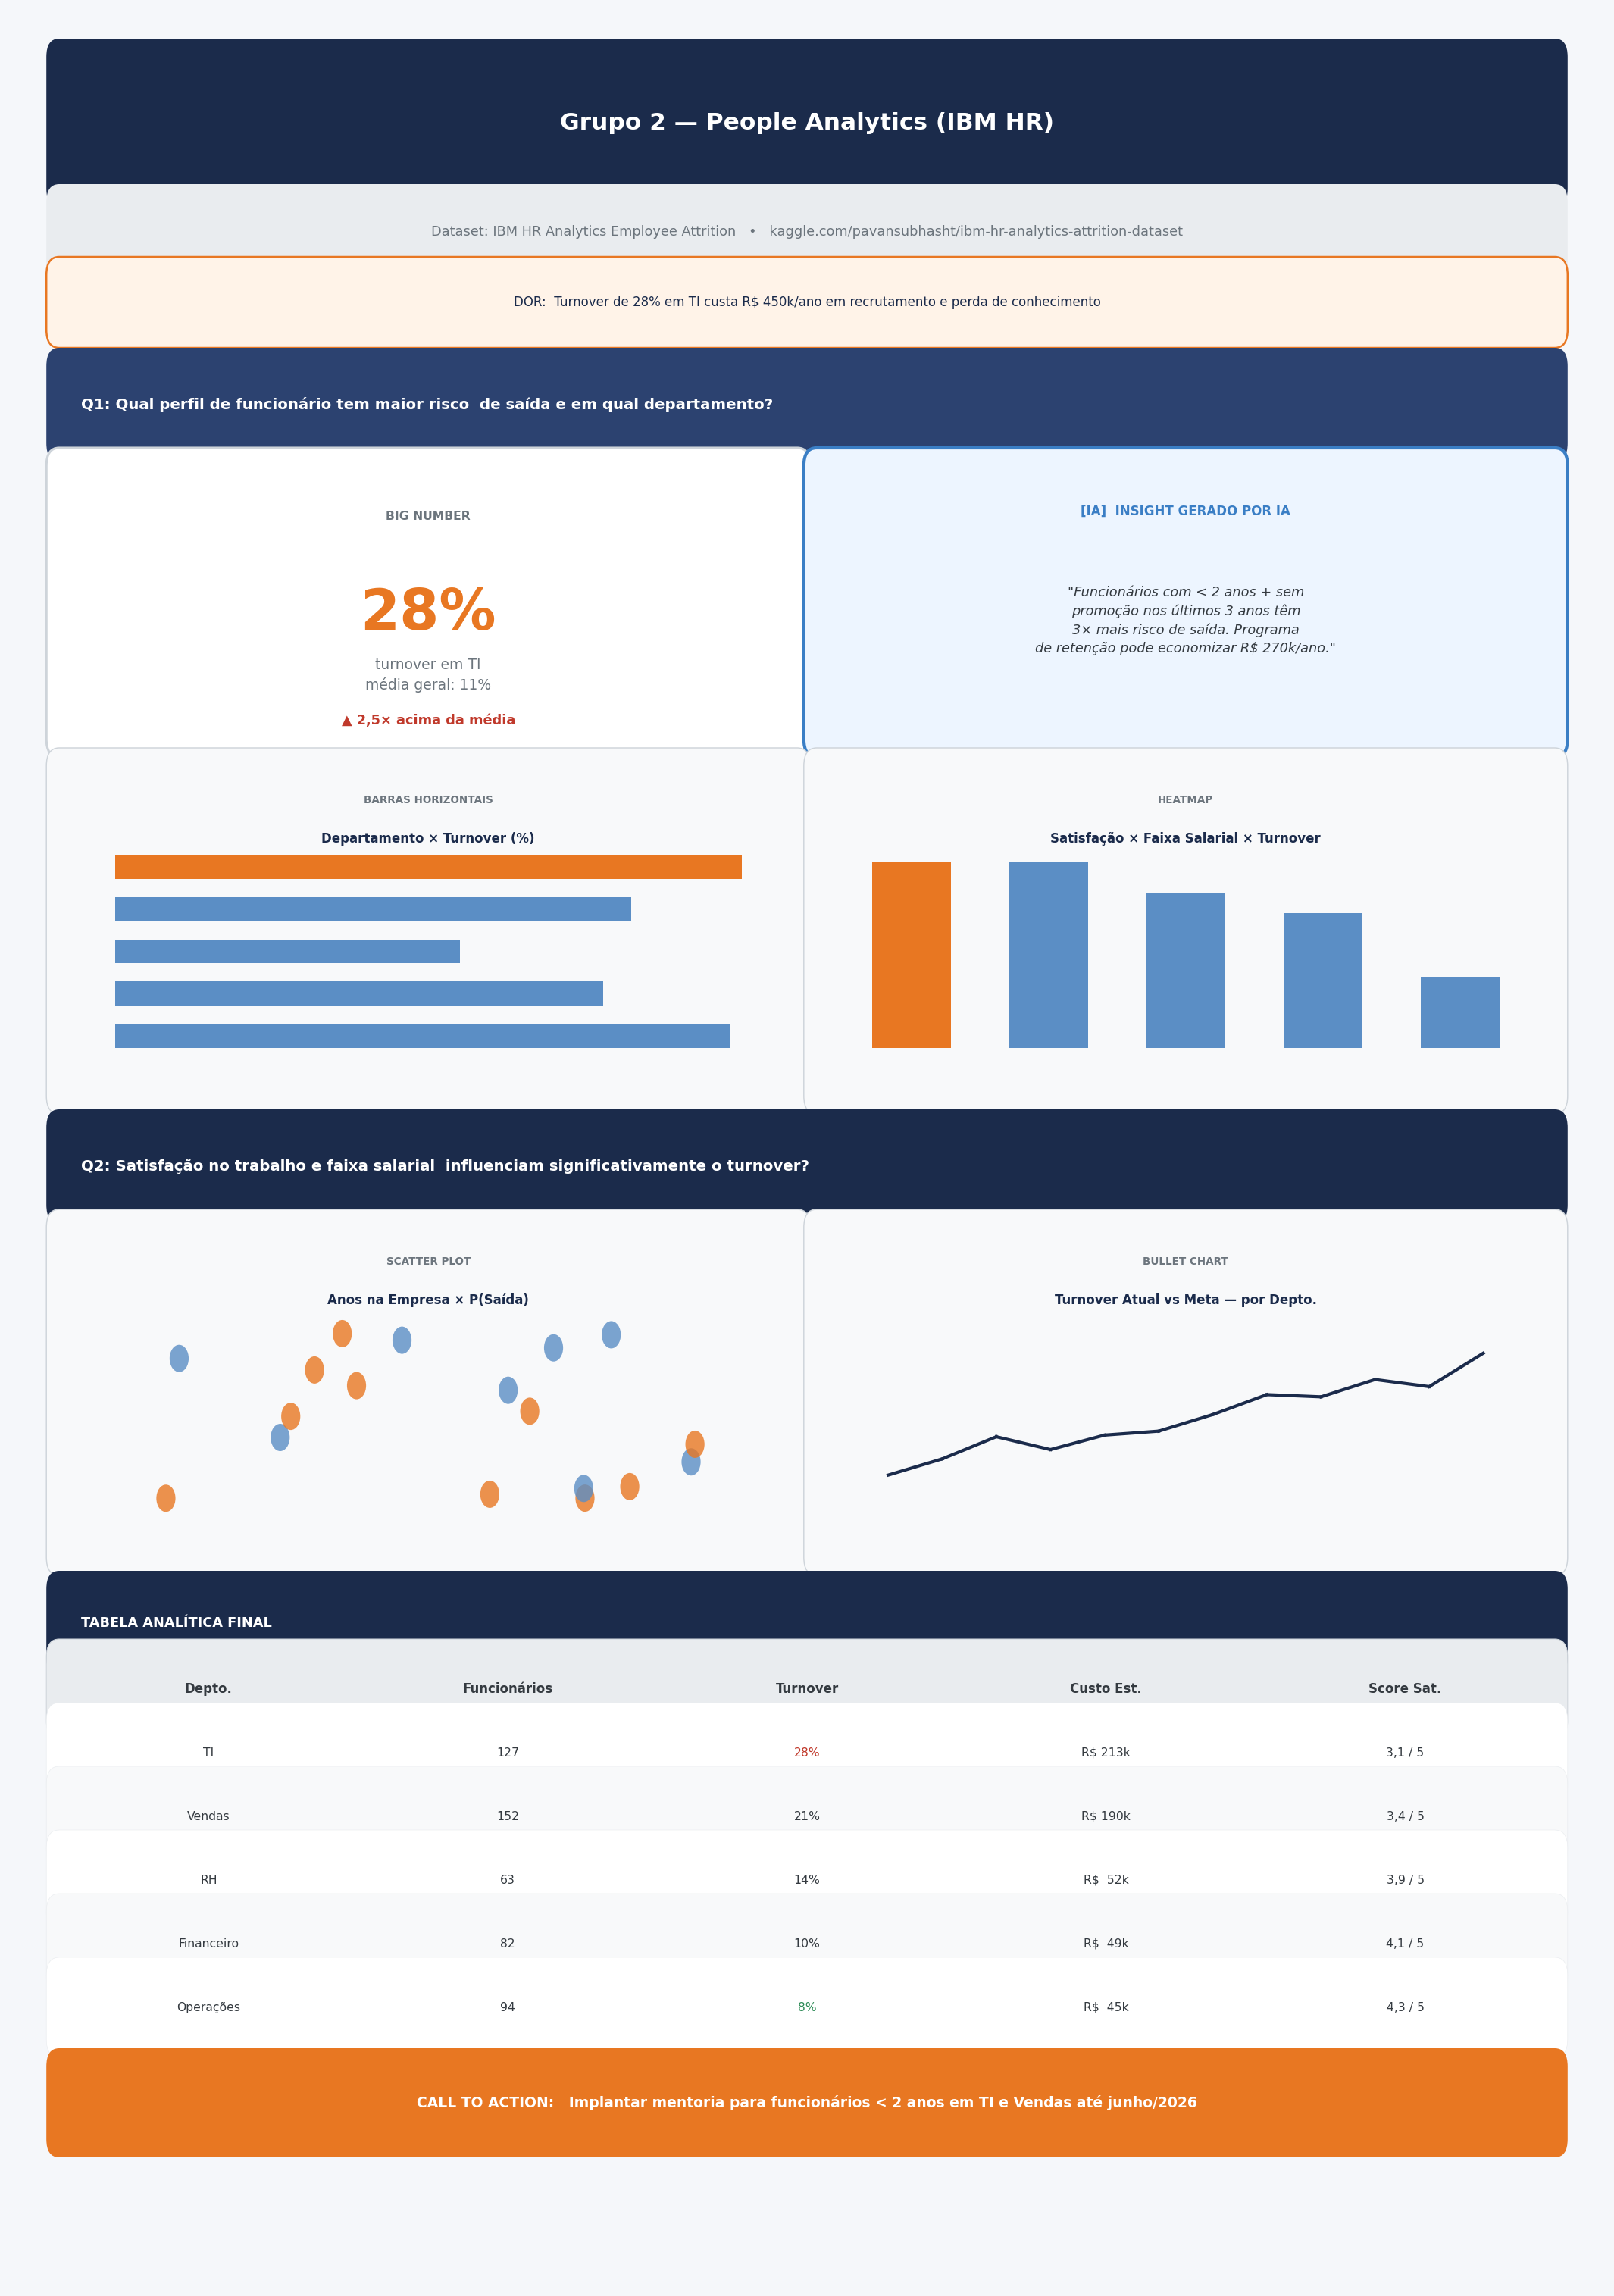
\includegraphics[width=\textwidth]{wireframes/wireframe_grupo2_rh_ibm.png}
\caption{Protótipo do dashboard — Grupo 2 (People Analytics IBM HR).}
\end{figure}

% =============================================================================
\section{Grupo 3 — Varejo: Superstore Dataset}
% =============================================================================

\begin{BoardBox}
\textbf{Briefing do Grupo 3}

\textbf{Dataset:} Sample Superstore Dataset\\
\textbf{Link:} \url{https://www.kaggle.com/datasets/vivek468/superstore-dataset-final}

\textbf{Dor de Negócio:} margens negativas em Tecnologia na Região Sul drenam
R\$120k/trimestre do lucro operacional.

\textbf{Pergunta 1:} ``Quais combinações de subcategoria de produto e região geram
prejuízo consistente?''

\textbf{Pergunta 2:} ``Existe correlação entre nível de desconto aplicado e margem
negativa?''

\textbf{Big Idea sugerida:} ``Descontos acima de 20\% em Máquinas e Copiadoras na
Região Sul concentram 73\% do prejuízo — capear o desconto em 12\% pode reverter a
margem de $-$4,2\% para $+$5,8\%, gerando R\$85k adicionais por trimestre.''

\textbf{Call to Action:} implementar política de desconto máximo de 12\% em Tecnologia
na Região Sul a partir do próximo trimestre.
\end{BoardBox}

\begin{SolvedBox}
\textbf{Transformações necessárias:}

\begin{enumerate}
  \item \textbf{Margem \%:} campo calculado: \texttt{Margem\_Pct = SUM([Profit]) / SUM([Sales]) * 100}
  \item \textbf{Faixa de desconto:}
  \texttt{IF [Discount] = 0 THEN "Sem Desconto"}
  \texttt{ELSEIF [Discount] <= 0.10 THEN "0-10\%"}
  \texttt{ELSEIF [Discount] <= 0.20 THEN "10-20\%"}
  \texttt{ELSE "Acima de 20\%" END}
  \item \textbf{Flag de prejuízo:} \texttt{Prejuizo = IF [Profit] < 0 THEN "Prejuízo" ELSE "Lucro" END}
  \item \textbf{Filtro de relevância:} considerar apenas sub-categorias com $>$ 50 transações.
  \item \textbf{Região:} coluna \texttt{Region} já disponível — verificar se está em inglês
  (South, Central, East, West); criar alias se necessário.
\end{enumerate}

\textbf{Campos para o dashboard:} \texttt{Sub-Category}, \texttt{Region}, \texttt{Sales},
\texttt{Profit}, \texttt{Margem\_Pct}, \texttt{Discount}, \texttt{Faixa\_Desconto},
\texttt{Prejuizo}, \texttt{Order Date}.
\end{SolvedBox}

\begin{SolvedBox}
\textbf{Construção do dashboard no Tableau:}

\textbf{Sheet 1 — Big Number:} \texttt{Margem\_Pct} filtrado para
Sub-Category $\in$ \{Machines, Copiers\} e Region = South. Meta: parâmetro de 8\%.
Gap em vermelho (abaixo da meta).

\textbf{Sheet 2 — Mapa de Calor (Pergunta 1):}
\texttt{Sub-Category} nas Rows, \texttt{Region} nas Columns; cor por
\texttt{Margem\_Pct} (escala divergente: vermelho = negativo, verde = positivo).
Título: ``Máquinas/Sul: único quadrante com margem $< -$8\%''.

\textbf{Sheet 3 — Scatter Desconto × Lucro (Pergunta 2):}
\texttt{Discount} nas Columns, \texttt{Profit} nas Rows; cor por \texttt{Faixa\_Desconto};
linha de referência em 0 no eixo Y; linha vertical em 20\% no eixo X.
Título: ``Acima de 20\% de desconto: 89\% dos pontos abaixo do zero''.

\textbf{Sheet 4 — Barras Agrupadas por Região:}
\texttt{Sub-Category} nas Rows, \texttt{Margem\_Pct} nas Columns, cor por \texttt{Region}.
Filtrar para sub-categorias de Tecnologia.

\textbf{Sheet 5 — Linha Trimestral:}
\texttt{Order Date} (Quarter) nas Columns, \texttt{Margem\_Pct} nas Rows;
filtrado para Tecnologia/Sul; linha de meta com parâmetro.
\end{SolvedBox}

\begin{figure}[H]
\centering
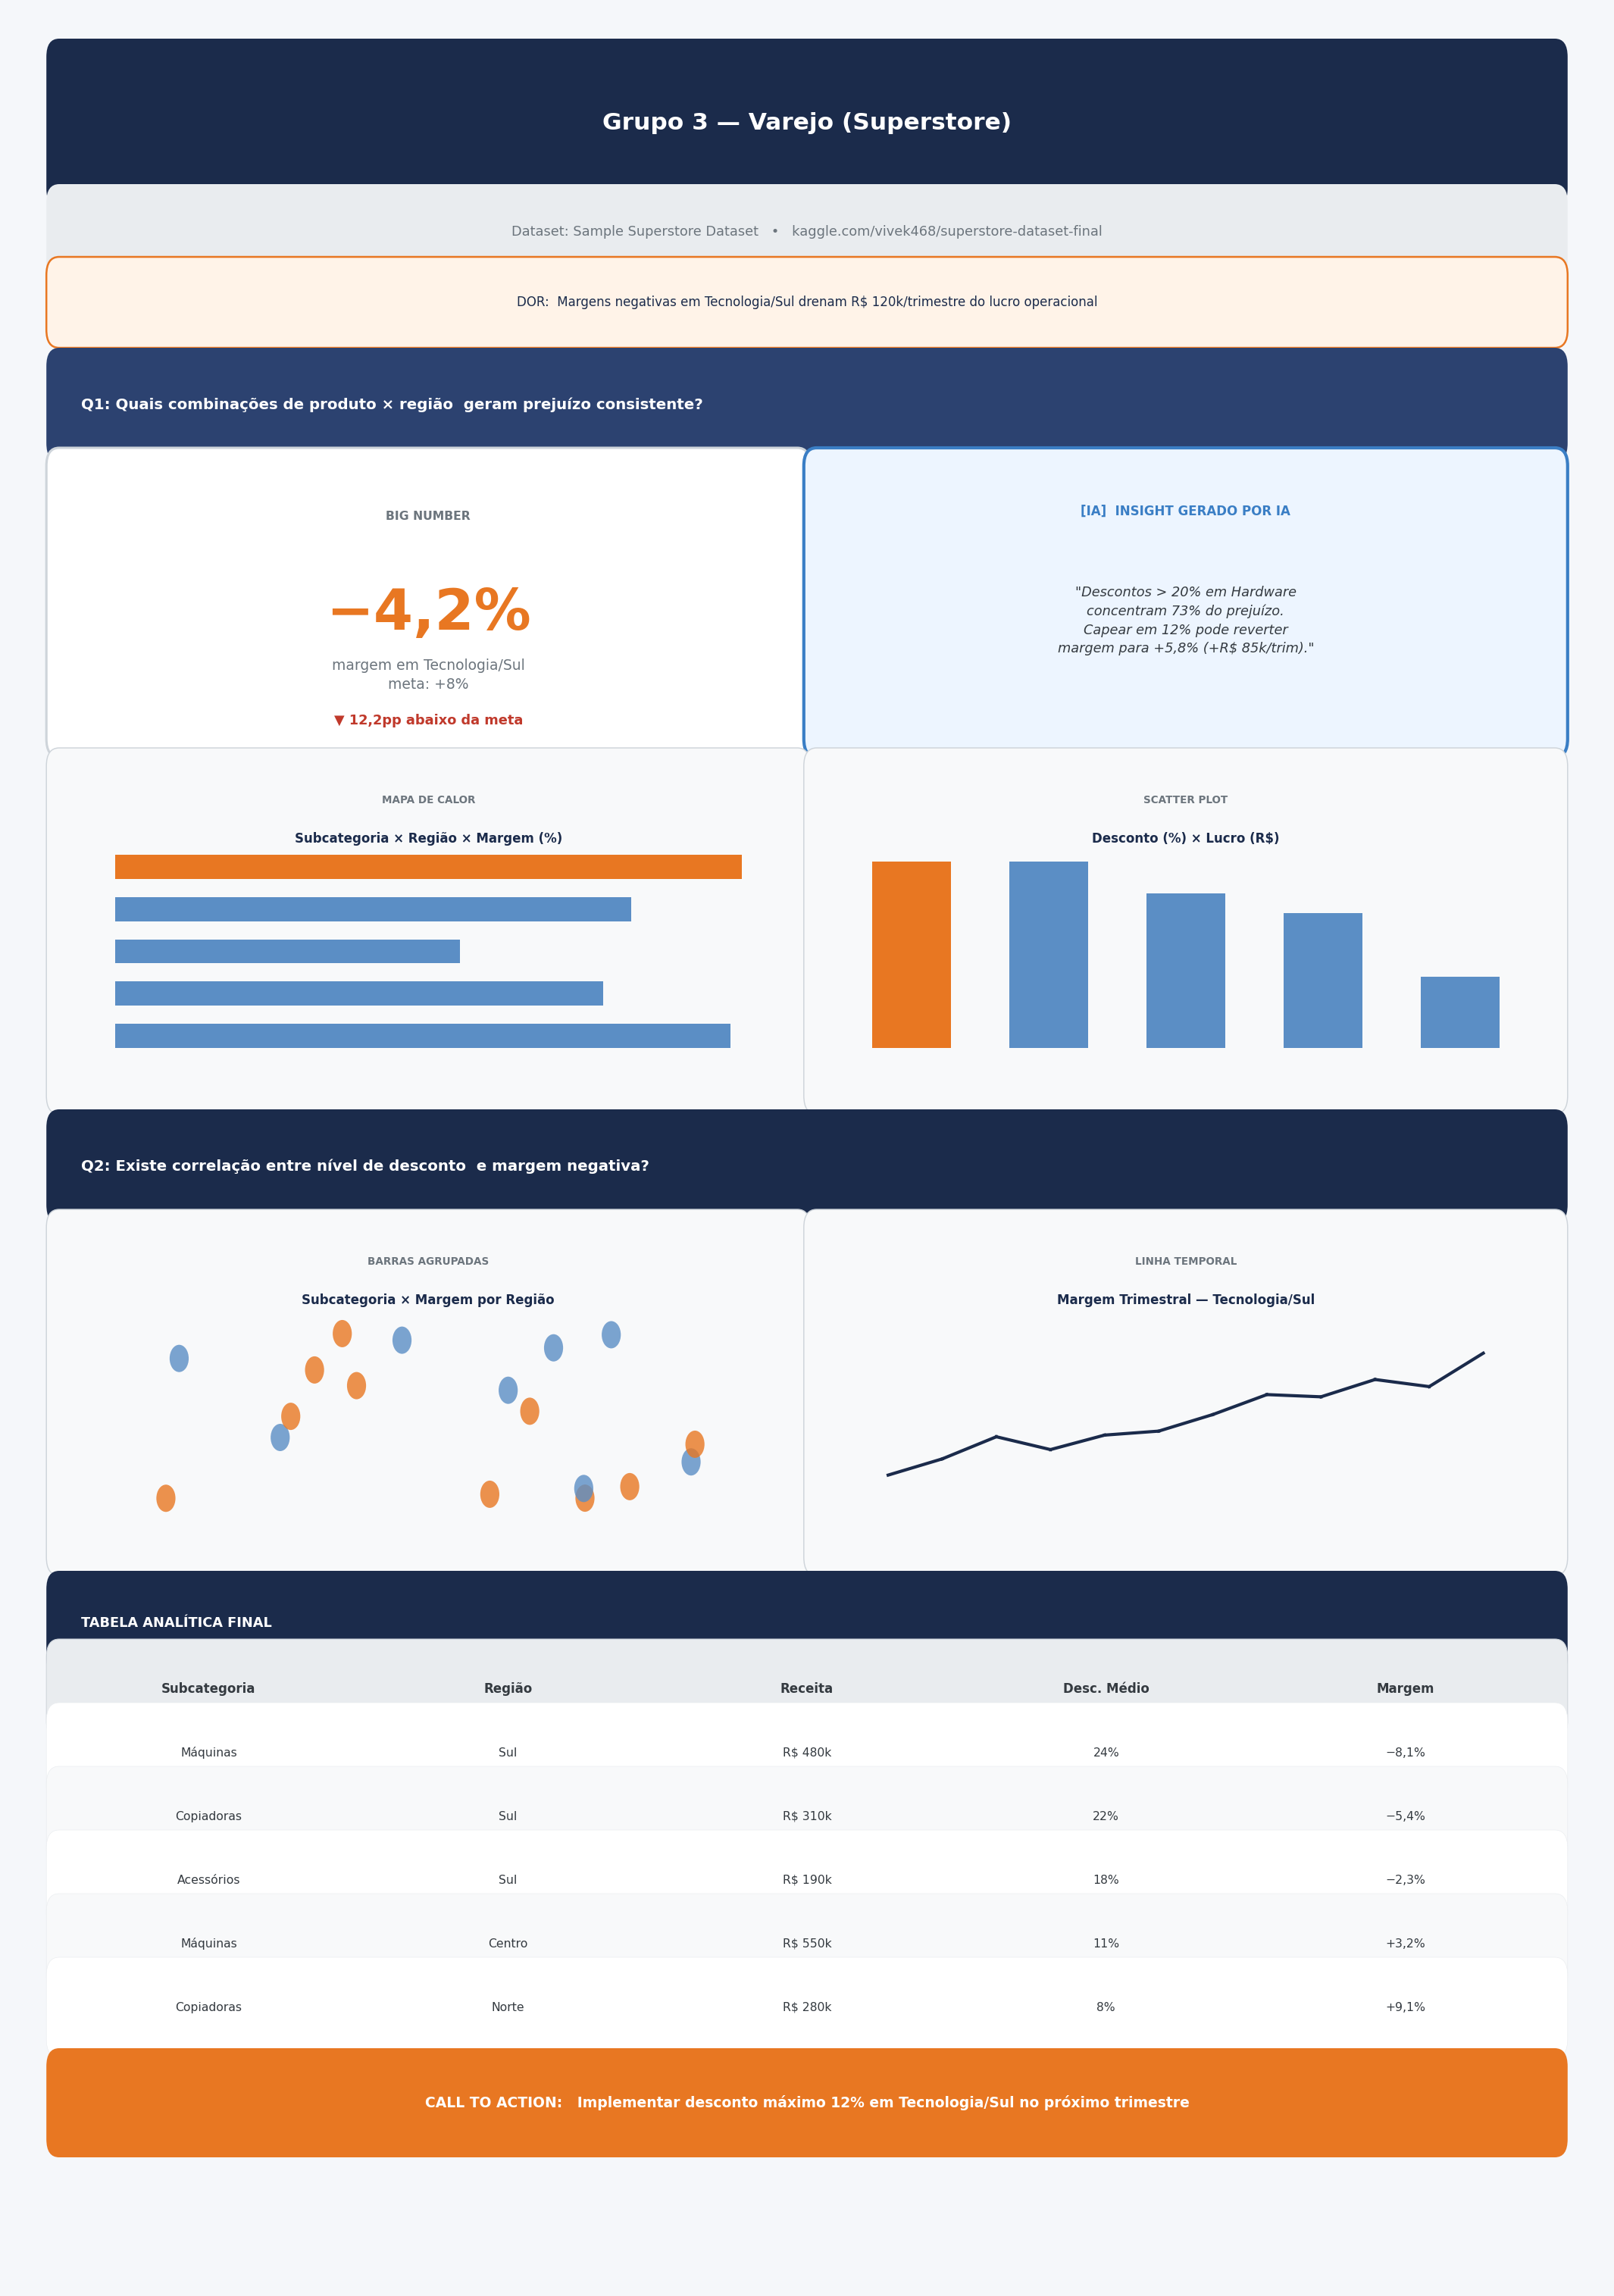
\includegraphics[width=\textwidth]{wireframes/wireframe_grupo3_superstore.png}
\caption{Protótipo do dashboard — Grupo 3 (Varejo Superstore).}
\end{figure}

% =============================================================================
\section{Grupo 4 — Saúde Pública: Heart Disease UCI}
% =============================================================================

\begin{BoardBox}
\textbf{Briefing do Grupo 4}

\textbf{Dataset:} Heart Disease UCI Dataset\\
\textbf{Link:} \url{https://www.kaggle.com/datasets/johnsmith88/heart-disease-dataset}

\textbf{Dor de Negócio:} doenças cardíacas representam 38\% das internações
hospitalares municipais, com custo médio de R\$12.000 por internação — sobrecarregando
o sistema de saúde público.

\textbf{Pergunta 1:} ``Quais fatores de risco têm maior correlação com diagnóstico
de doença cardíaca?''

\textbf{Pergunta 2:} ``Qual faixa etária e perfil clínico priorizar em campanhas
preventivas de baixo custo?''

\textbf{Big Idea sugerida:} ``Combinando colesterol $>$ 240 + pressão arterial $>$ 140
+ idade $>$ 55 anos, identificamos 73\% dos casos de alto risco com apenas 3 variáveis —
uma triagem preventiva focada nesse perfil pode reduzir internações em 25\% e gerar
economia de R\$2,1M/ano.''

\textbf{Call to Action:} implantar triagem preventiva gratuita semestral para
homens $>$ 55 anos com colesterol $>$ 240.
\end{BoardBox}

\begin{SolvedBox}
\textbf{Transformações necessárias:}

O dataset Heart Disease UCI usa variáveis codificadas numericamente. Decodificar:
\begin{enumerate}
  \item \textbf{Variável alvo:} \texttt{target} (0 = sem doença, 1 = doença).
  Campo calculado: \texttt{Diagnostico = IF [target]=1 THEN "Doença" ELSE "Sem Doença" END}
  \item \textbf{Sexo:} \texttt{sex} → \texttt{IF [sex]=1 THEN "Masculino" ELSE "Feminino" END}
  \item \textbf{Faixa etária:} \texttt{IF [age] < 45 THEN "< 45"}
  \texttt{ELSEIF [age] < 55 THEN "45–54"}
  \texttt{ELSEIF [age] < 65 THEN "55–64"}
  \texttt{ELSE "65+" END}
  \item \textbf{Perfil de risco:}
  \texttt{IF [chol] > 240 AND [trestbps] > 140 AND [age] > 55}
  \texttt{THEN "Alto Risco" ELSE "Normal" END}
  \item \textbf{Taxa de doença:} \texttt{Taxa\_Doenca = AVG(target) * 100}
  \item \textbf{Tipo de dor no peito:} \texttt{cp} (0–3) → decodificar como:
  0=Assintomático, 1=Angina Típica, 2=Angina Atípica, 3=Não-Anginosa.
\end{enumerate}

\textbf{Campos para o dashboard:} \texttt{Diagnostico}, \texttt{Sexo},
\texttt{Faixa\_Etaria}, \texttt{chol} (colesterol), \texttt{trestbps} (pressão),
\texttt{age}, \texttt{Perfil\_Risco}, \texttt{Taxa\_Doenca}.
\end{SolvedBox}

\begin{SolvedBox}
\textbf{Construção do dashboard no Tableau:}

\textbf{Sheet 1 — Big Number:} \texttt{Taxa\_Doenca} filtrado por
\texttt{Sexo = "Masculino"} e \texttt{Faixa\_Etaria = "55–64"} ou \texttt{"65+"}.
Fonte 28pt, laranja.

\textbf{Sheet 2 — Barras por Fator de Risco (Pergunta 1):}
Criar campo de correlação calculada para: \texttt{chol}, \texttt{trestbps},
\texttt{thalach} (freq. cardíaca máx.), \texttt{age}, \texttt{cp}.
Apresentar em barras horizontais ordenadas por magnitude.
Título: ``Pressão arterial e colesterol: maiores preditores''.

\textbf{Sheet 3 — Heatmap Faixa Etária × Fatores (Pergunta 2):}
\texttt{Faixa\_Etaria} nas Columns, \texttt{Perfil\_Risco} nas Rows;
cor por \texttt{Taxa\_Doenca}; escala verde→vermelho.

\textbf{Sheet 4 — Scatter Colesterol × Pressão (Pergunta 2):}
\texttt{chol} nas Columns, \texttt{trestbps} nas Rows;
cor por \texttt{Diagnostico} (laranja = doença, cinza = sem doença);
linhas de referência em 240 (colesterol) e 140 (pressão).
Título: ``Quadrante crítico: colesterol $>$ 240 + pressão $>$ 140''.

\textbf{Sheet 5 — Boxplot por Grupo (Pergunta 2):}
\texttt{Diagnostico} nas Columns, \texttt{age} nas Rows;
Box and Whisker Plot via Tableau (Show Me).
Título: ``Grupo com doença: mediana de X anos — 8 anos mais velho''.
\end{SolvedBox}

\begin{figure}[H]
\centering
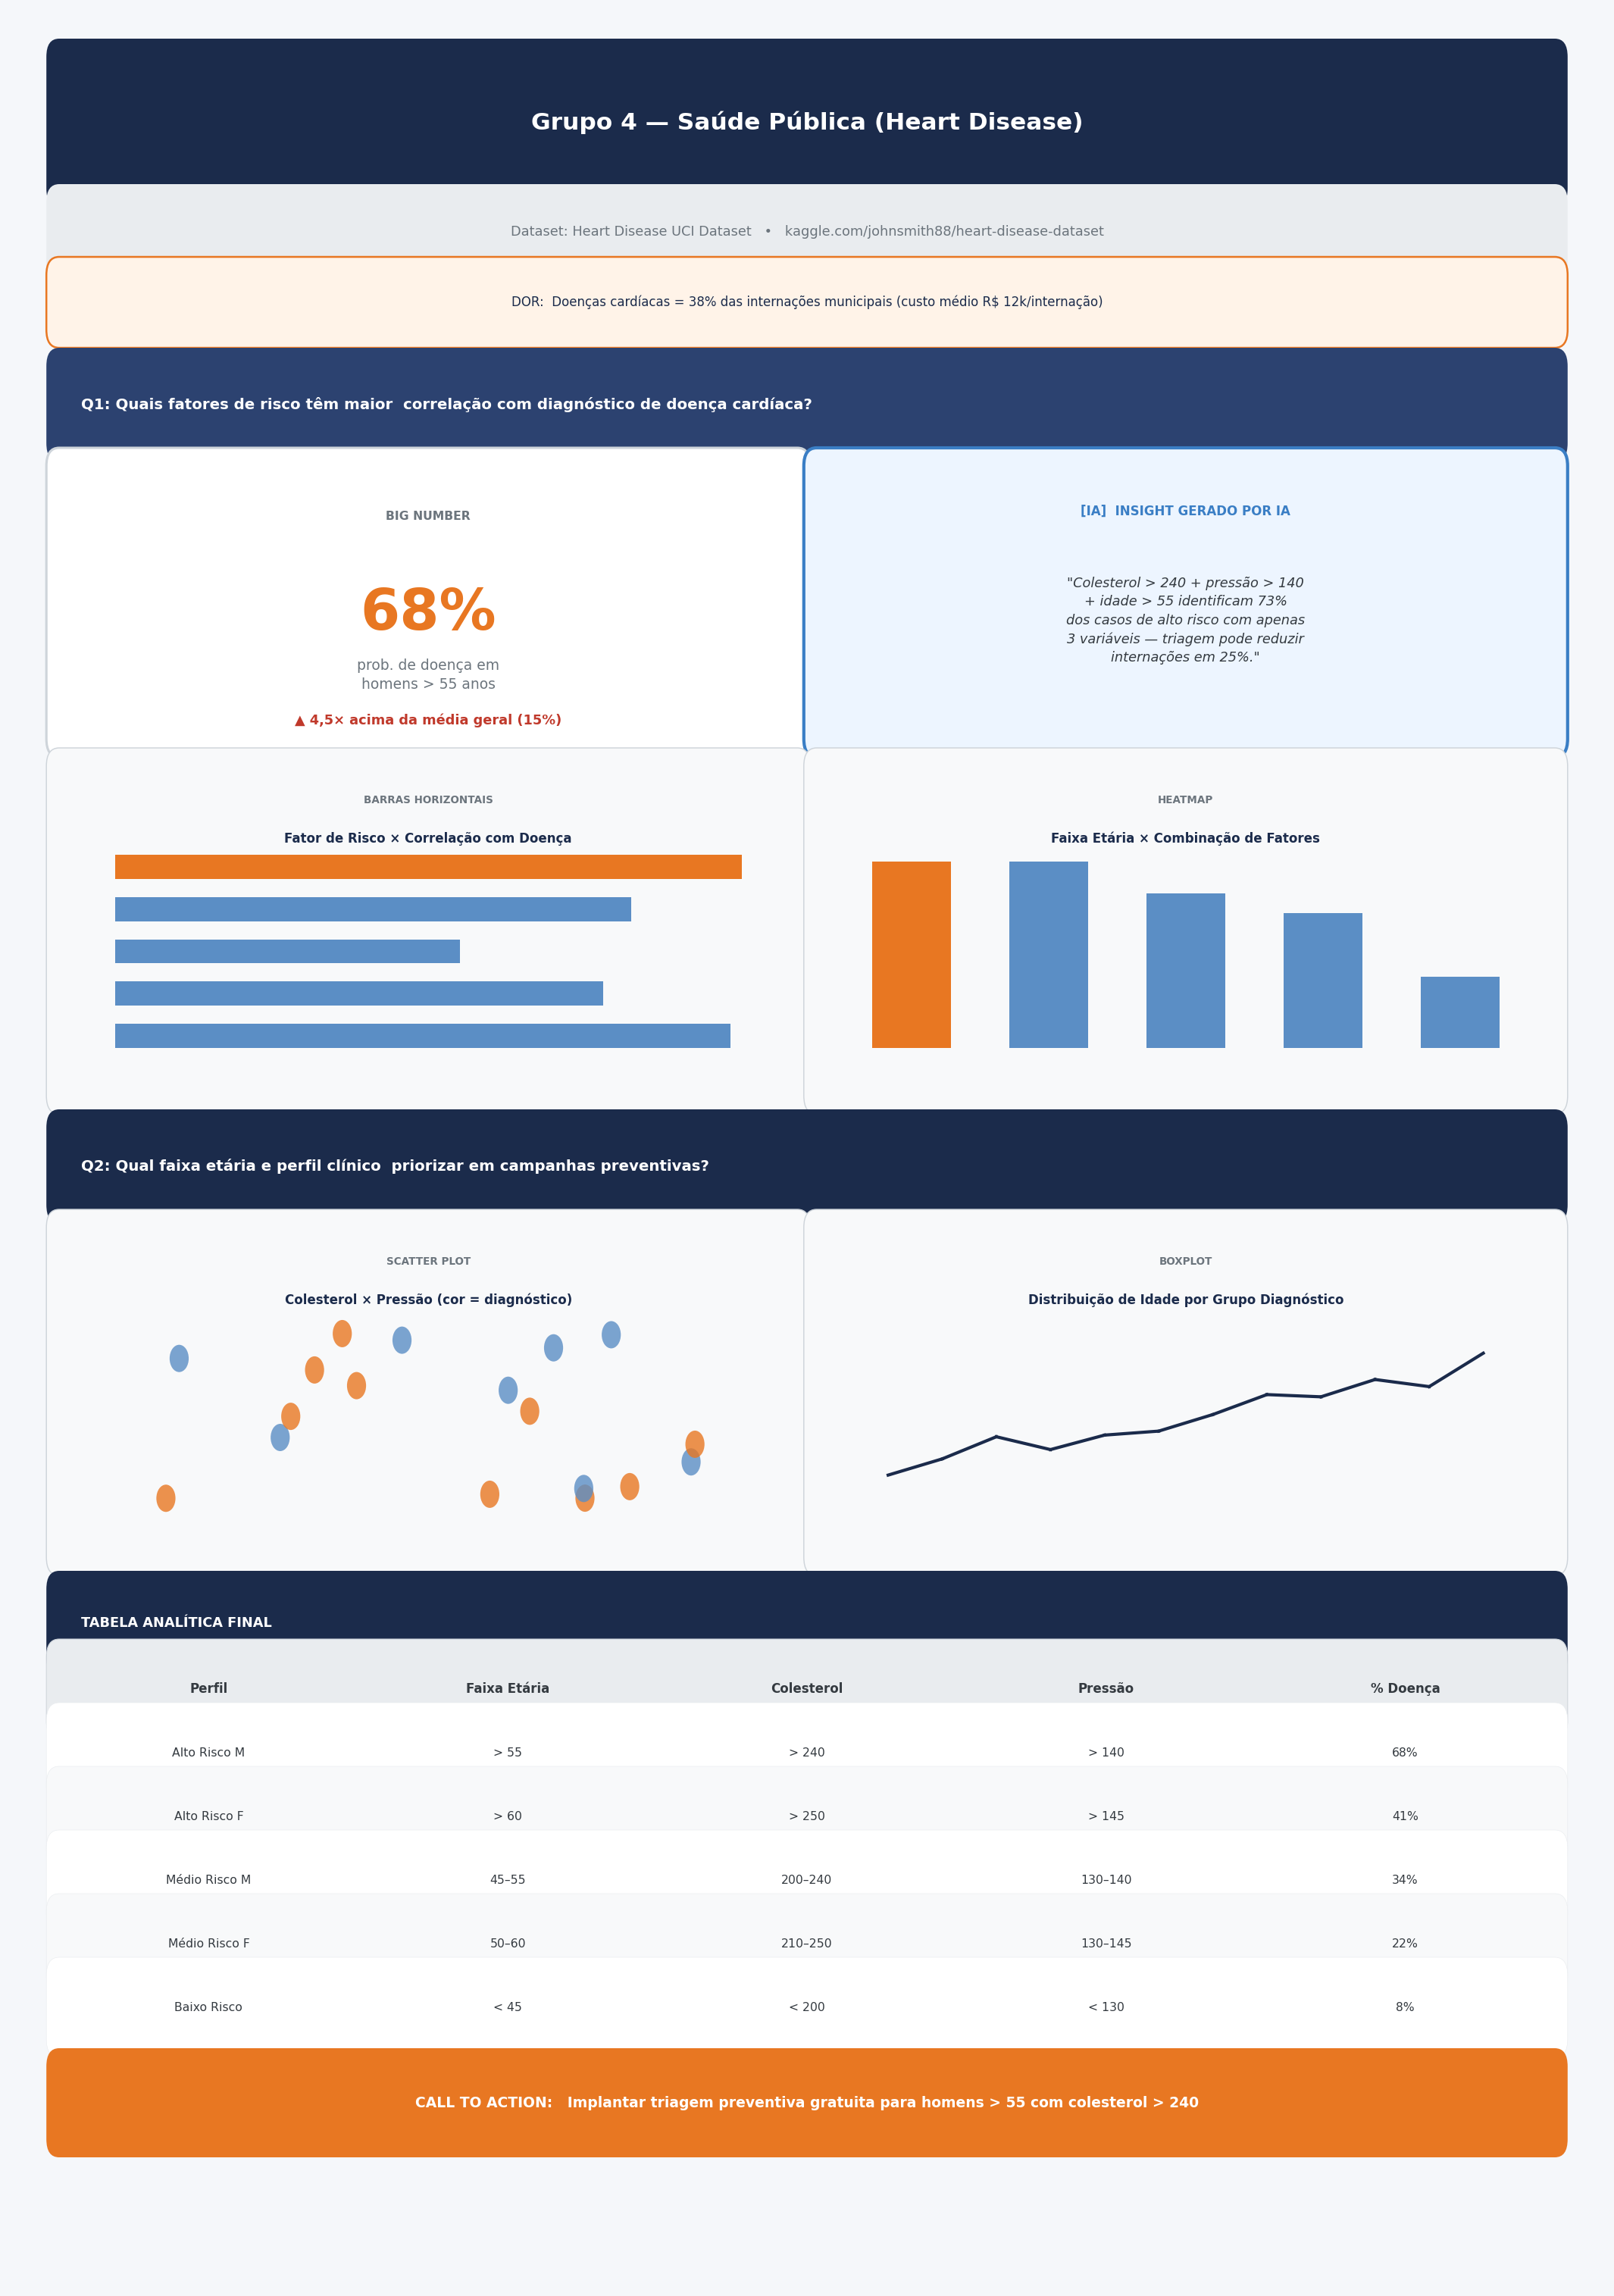
\includegraphics[width=\textwidth]{wireframes/wireframe_grupo4_saude.png}
\caption{Protótipo do dashboard — Grupo 4 (Saúde Pública Heart Disease).}
\end{figure}

% =============================================================================
\section{Grupo 5 — Fintech: Credit Card Customers (Churn)}
% =============================================================================

\begin{BoardBox}
\textbf{Briefing do Grupo 5}

\textbf{Dataset:} Credit Card Customers Dataset\\
\textbf{Link:} \url{https://www.kaggle.com/datasets/sakshigoyal7/credit-card-customers}

\textbf{Dor de Negócio:} churn de cartão Premium custa R\$2,1M/ano em receita perdida
de juros e anuidade.

\textbf{Pergunta 1:} ``Qual perfil de cliente Premium tem maior propensão ao
cancelamento?''

\textbf{Pergunta 2:} ``Frequência de uso e limite de crédito influenciam
significativamente o churn?''

\textbf{Big Idea sugerida:} ``Clientes Premium com limite $<$ R\$10k e menos de
20 transações por ano têm 4$\times$ mais chance de cancelamento — um programa de
engajamento proativo focado nesse perfil pode preservar R\$1,2M em receita anual.''

\textbf{Call to Action:} lançar campanha de reativação para Premium com limite
$<$ R\$10k e $<$ 20 transações/ano — início imediato.
\end{BoardBox}

\begin{SolvedBox}
\textbf{Transformações necessárias:}

\begin{enumerate}
  \item \textbf{Variável alvo:} \texttt{Attrition\_Flag} (``Attrited Customer'' vs
  ``Existing Customer'') → campo calculado:
  \texttt{Churned = IF [Attrition\_Flag]="Attrited Customer" THEN 1 ELSE 0 END}
  \item \textbf{Taxa de churn:} \texttt{Churn\_Rate = AVG(Churned) * 100}
  \item \textbf{Faixa de limite:}
  \texttt{IF [Credit\_Limit] < 10000 THEN "< R\$10k"}
  \texttt{ELSEIF [Credit\_Limit] < 30000 THEN "R\$10k–30k"}
  \texttt{ELSE "> R\$30k" END}
  \item \textbf{Frequência de uso:}
  \texttt{IF [Total\_Trans\_Ct] < 20 THEN "Baixa (< 20)"}
  \texttt{ELSEIF [Total\_Trans\_Ct] < 50 THEN "Média (20–50)"}
  \texttt{ELSE "Alta (> 50)" END}
  \item \textbf{Taxa de utilização:}
  \texttt{Utilizacao = [Total\_Revolving\_Bal] / [Credit\_Limit]}
  \item \textbf{Perfil de risco:}
  \texttt{IF [Total\_Trans\_Ct] < 20 AND [Faixa\_Limite]="< R\$10k"}
  \texttt{THEN "Alto Risco" ELSE "Normal" END}
\end{enumerate}

\textbf{Campos para o dashboard:} \texttt{Attrition\_Flag}, \texttt{Churn\_Rate},
\texttt{Faixa\_Limite}, \texttt{Freq\_Uso}, \texttt{Credit\_Limit},
\texttt{Total\_Trans\_Ct}, \texttt{Total\_Trans\_Amt}, \texttt{Perfil\_Risco}.
\end{SolvedBox}

\begin{SolvedBox}
\textbf{Construção do dashboard no Tableau:}

\textbf{Sheet 1 — Big Number:} \texttt{Churn\_Rate} filtrado para
\texttt{Faixa\_Limite = "< R\$10k"} e \texttt{Card\_Category = "Platinum"} ou similar.

\textbf{Sheet 2 — Barras por Faixa de Limite (Pergunta 1):}
\texttt{Faixa\_Limite} nas Rows, \texttt{Churn\_Rate} nas Columns;
linha de referência com o benchmark de 8\%;
destacar a barra de $<$ R\$10k em laranja.
Título: ``Clientes com limite $<$ R\$10k: churn 3,2$\times$ acima do benchmark''.

\textbf{Sheet 3 — Scatter Frequência × Valor Médio (Pergunta 1):}
\texttt{Total\_Trans\_Ct} nas Columns, \texttt{Total\_Trans\_Amt} nas Rows;
cor por \texttt{Attrition\_Flag} (laranja = churn, cinza = ativo);
linha vertical em 20 transações (zona de risco).
Título: ``Clientes com $<$ 20 transações: zona de alto risco''.

\textbf{Sheet 4 — Linha Temporal de Churn por Segmento (Pergunta 2):}
Agrupar por \texttt{Freq\_Uso}; se não houver data disponível, usar
\texttt{Months\_on\_book} como proxy de tempo.

\textbf{Sheet 5 — Heatmap Atividade × Limite (Pergunta 2):}
\texttt{Faixa\_Limite} nas Columns, \texttt{Freq\_Uso} nas Rows;
cor por \texttt{Churn\_Rate}; escala verde→vermelho.
\end{SolvedBox}

\begin{figure}[H]
\centering
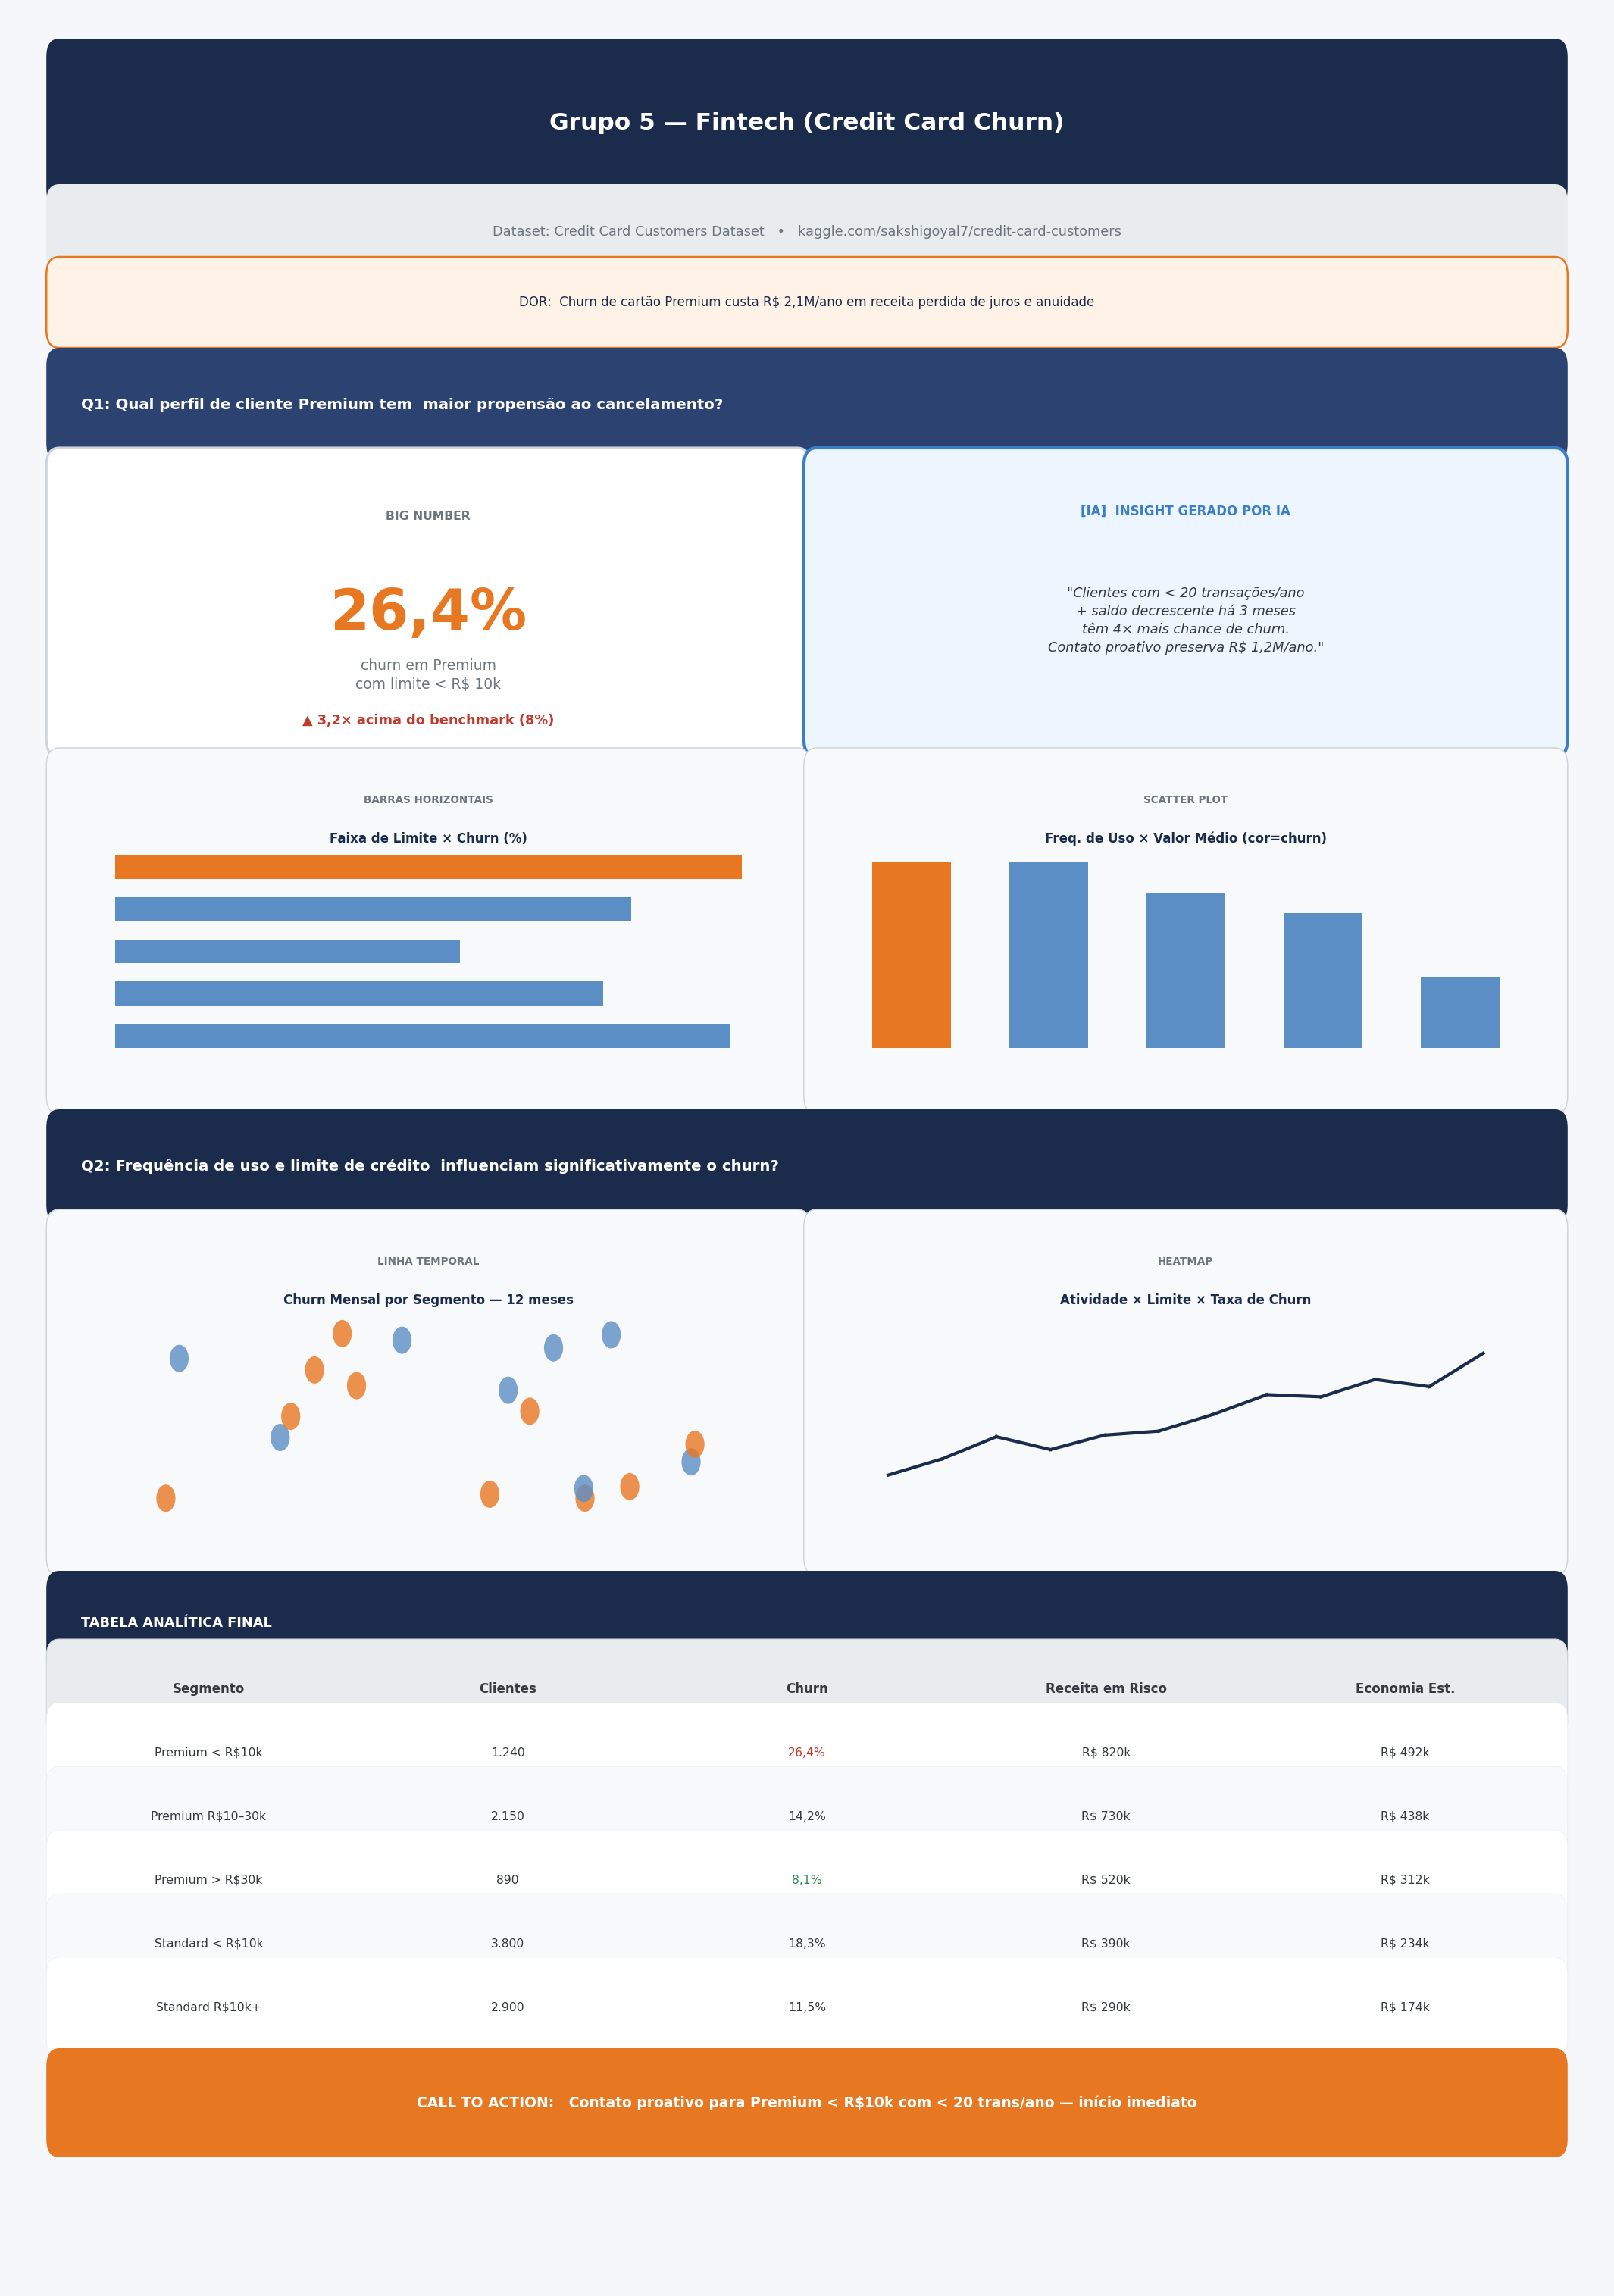
\includegraphics[width=\textwidth]{wireframes/wireframe_grupo5_fintech.png}
\caption{Protótipo do dashboard — Grupo 5 (Fintech Credit Card Churn).}
\end{figure}

% =============================================================================
\section{Critérios de Avaliação}
% =============================================================================

\begin{BoardBox}
\textbf{Rubrica de avaliação — Apresentação em Grupo (18/05)}

\begin{tabular}{|p{4.5cm}|r|p{7cm}|}
\hline
\textbf{Critério} & \textbf{Peso} & \textbf{Descrição} \\
\hline
Big Idea formulada & 15\% & 1 frase: ponto de vista + tensão + stake; explicitada no pitch \\
Estrutura do dashboard & 20\% & Pergunta → Big Number + Insight IA → Gráficos → Tabela \\
Qualidade dos visuais & 20\% & Títulos-mensagem; cor com propósito; sem chartjunk \\
Insight IA & 15\% & Presente ao lado do Big Number; acionável; não genérico \\
Tableau funcional & 15\% & Pelo menos 1 filtro ou parâmetro funcionando \\
Pitch 3 minutos & 15\% & SCR completo; dentro do tempo; call to action explícito \\
\hline
\textbf{Total} & \textbf{100\%} & \\
\hline
\end{tabular}
\end{BoardBox}

\begin{NoteBox}
\textbf{Formato da apresentação:}
\begin{itemize}
  \item \textbf{Tempo:} 3 minutos de pitch + 2 minutos de perguntas da turma
  \item \textbf{Ordem:} sorteio na abertura da aula
  \item \textbf{Obrigatório:} o Tableau Public deve estar aberto antes de começar
  (link compartilhado no chat com o professor)
  \item \textbf{Enquanto os outros grupos apresentam:} cada aluno anota em papel:\\
  (1) Big Idea em 1 frase do que ouviu; (2) uma decisão que tomaria;
  (3) uma sugestão de melhoria — exercício de escuta ativa.
\end{itemize}
\end{NoteBox}

% =============================================================================
\section{Prompt Reutilizável — Geração de Insight por IA}
% =============================================================================

\begin{BoardBox}
\textbf{Prompt para gerar o Insight IA no ChatGPT / Gemini}

Cole o prompt abaixo no ChatGPT ou Gemini, substituindo os campos entre colchetes:

\medskip
\begin{quote}
\textit{``Você é um analista de dados sênior especializado em [ÁREA DO NEGÓCIO].
Com base nos dados abaixo, gere UM insight acionável em no máximo 3 linhas.
O insight deve: (1) identificar um padrão não óbvio ou contraintuitivo nos dados,
(2) quantificar o impacto com número concreto (percentual, valor financeiro ou
comparação com benchmark), e (3) propor uma ação específica com estimativa de
resultado mensurável.

Contexto do negócio: [DESCREVA A DOR DO SEU GRUPO EM 1 FRASE].
Pergunta que o dashboard responde: [PERGUNTA DE NEGÓCIO DO GRUPO].
Dados principais: [COLE AQUI O RESUMO DOS DADOS — ex.: top 5 linhas da tabela analítica].

Formato de saída: uma única frase de insight entre aspas, iniciando com o dado
mais impactante.''}
\end{quote}

\medskip
\textbf{Exemplo de resultado esperado:}\\
\textit{``Eletrônicos concentram 2,4$\times$ mais atrasos que a média geral —
priorizar SLA nessa categoria pode aumentar o review score de 3,2 para 4,1 estrelas
e reduzir o churn de vendedores em 15\%.''}
\end{BoardBox}
